\documentclass{article}
\usepackage[utf8]{inputenc}
\usepackage{amsmath}
\usepackage{amssymb}
\usepackage{graphicx}
\usepackage{xcolor}

\begin{document}
\section*{Structured linear systems with pivoting}
We are given the following block partitioned linear system od equations
\begin{equation*}
    \mathbf{A}\mathbf{x} = \mathbf{b}\,,\quad \mathbf{A} = \begin{bmatrix}
    \mathbf{D}_{1} & \mathbf{C}_{1} \\ \mathbf{C} & \mathbf{D}_{2}
    \end{bmatrix}
\end{equation*}
where all the $n \times n$ matrices $\mathbf{D}_{1}$, $\mathbf{D}_{2}$ and $\mathbf{C}$ are diagonal. We can thus describe the matrices using three $n$-vectors $\mathbf{d}_{1}$, $\mathbf{c}$ and $\mathbf{d}_{2}$ which provide the diagonal of the matrix blocks. 

\subsection*{2-2.a}
We are tasked with finding the permutations of rows and columns that convert the matrix into a \textbf{tridiagonal} matrix. Let us first consider an example to illustrate how the block partitioned linear system of equations looks like
\begin{equation*}
\mathbf{A} = 
    \begin{bmatrix}
        d_{1,1}  & 0 & c_{1}  & 0 \\
        0 & d_{1,2}  & 0 & c_{2}  \\
        c_{1} & 0 & d_{2,1} & 0 \\
        0 & c_{2}  & 0 & d_{2,2}  
    \end{bmatrix}
\end{equation*}
We now perform the following swap of rows and columns
\begin{equation*}
    \begin{bmatrix}
        d_{1,1}  & 0 & c_{1}  & 0 \\
        \mathbf{0} & \mathbf{d_{1,2}}  & \mathbf{0} & \mathbf{c_{2}}  \\
        \mathbf{c_{1}} & \mathbf{0} & \mathbf{d_{2,1}} & \mathbf{0} \\
        0 & c_{2}  & 0 & d_{2,2}  
    \end{bmatrix} \longrightarrow
    \begin{bmatrix}
        d_{1,1}  & \mathbf{0} & \mathbf{c_{1}}  & 0 \\
        c_{1} & \mathbf{0} & \mathbf{d_{2,1}} & 0 \\
                0 & \mathbf{d_{1,2}}  & \mathbf{0} & c_{2}  \\
        0 & \mathbf{c_{2}}  & \mathbf{0} & d_{2,2}  
    \end{bmatrix}  \longrightarrow 
    \begin{bmatrix}
        d_{1,1} & c_{1} & 0 & 0 \\
        c_{1} & c_{2,1} & 0 & 0 \\
        0 & 0 & d_{1,2} & c_{2} \\
        0 & 0 & c_{2} & d_{2,2}
    \end{bmatrix}
\end{equation*}
We now have a different block partitioned linear system of equations composed of the two blocks
\begin{equation*}
    \mathbf{B}_{1} = \begin{bmatrix}
        d_{1,1} & c_{1} \\
        c_{1} & c_{2,1} 
    \end{bmatrix} \quad \mathbf{B}_{2} = \begin{bmatrix}
        d_{1,2} & c_{2} \\
        c_{2} & d_{2,2}
    \end{bmatrix} \quad \tilde{\mathbf{A}} = \begin{bmatrix}
        \mathbf{B}_{1} & \mathbf{O} \\
        \mathbf{O} & \mathbf{B}_{2}
    \end{bmatrix}
\end{equation*}
which is indeed tridiagonal, however this would not directly work with larger blocks, so let us consider the $3 \times 3$ case.
\begin{equation*}
    \begin{bmatrix}
        d_{1,1}  & \mathbf{0} & 0 & \mathbf{c_{1}}  & 0 & 0 \\
        0 & \mathbf{d_{1,2}} & 0  & \mathbf{0} & c_{2}  & 0 \\
        0 & \mathbf{0} & d_{1,3} & \mathbf{0} & 0 & c_{3} \\
        c_{1} & \mathbf{0} & 0& \mathbf{d_{2,1}} & 0 & 0 \\
        0 & \mathbf{c_{2}}  & 0 & \mathbf{0} & d_{2,2}  & 0 \\
        0 & \mathbf{0} & c_{3} & \mathbf{0} & 0 & d_{2,3}
    \end{bmatrix} \longrightarrow \begin{bmatrix}
        d_{1,1}  & c_{1} & \mathbf{0} & 0 & \mathbf{0} & 0 \\
        0 & 0  & \mathbf{0} & d_{1,2} & \mathbf{c_{2}}  & 0 \\
        0 & 0 & \mathbf{d_{1,3}}& 0 & \mathbf{0} & c_{3} \\
        c_{1} & d_{2,1} & \mathbf{0}& 0 & \mathbf{0} & 0 \\
        0 & 0 & \mathbf{0} & c_{2} & \mathbf{d_{2,2}}  & 0 \\
        0 & 0 & \mathbf{c_{3}} & 0 & \mathbf{0} & d_{2,3}
    \end{bmatrix} 
\end{equation*}

\pagebreak

\begin{equation*}
\begin{bmatrix}
        d_{1,1}  & c_{1} & \mathbf{0} & 0 & \mathbf{0} & 0 \\
        0 & 0  & \mathbf{0} & d_{1,2} & \mathbf{c_{2}}  & 0 \\
        0 & 0 & \mathbf{d_{1,3}}& 0 & \mathbf{0} & c_{3} \\
        c_{1} & d_{2,1} & \mathbf{0}& 0 & \mathbf{0} & 0 \\
        0 & 0 & \mathbf{0} & c_{2} & \mathbf{d_{2,2}}  & 0 \\
        0 & 0 & \mathbf{c_{3}} & 0 & \mathbf{0} & d_{2,3}
    \end{bmatrix} \longrightarrow
    \begin{bmatrix}
        d_{1,1}  & c_{1} & 0 & 0 & 0& 0 \\
        0 & 0  & c_{2} & d_{1,2} & 0  & 0 \\
        0 & 0 & 0& 0 & d_{1,3} & c_{3} \\
        c_{1} & d_{2,1} & 0& 0 & 0 & 0 \\
        0 & 0 & d_{2,2} & c_{2} & 0  & 0 \\
        0 & 0 & 0 & 0 & c_{3} & d_{2,3}
    \end{bmatrix} 
\end{equation*}
\begin{equation*}
\begin{bmatrix}
        d_{1,1}  & c_{1} & 0 & 0 & 0& 0 \\
        \mathbf{0} & \mathbf{0}  & \mathbf{c_{2}} & \mathbf{d_{1,2}} & \mathbf{0}  & \mathbf{0} \\
        0 & 0 & 0& 0 & d_{1,3} & c_{3} \\
        \mathbf{c_{1}} & \mathbf{d_{2,1}} & \mathbf{0}& \mathbf{0} & \mathbf{0} & \mathbf{0} \\
        0 & 0 & d_{2,2} & c_{2} & 0  & 0 \\
        0 & 0 & 0 & 0 & c_{3} & d_{2,3}
    \end{bmatrix} \longrightarrow 
\begin{bmatrix}
        d_{1,1}  & c_{1} & 0 & 0 & 0& 0 \\
        c_{1} & d_{2,1}  & 0 & 0 & 0  & 0 \\
        0 & 0 & 0& 0 & d_{1,3} & c_{3} \\
        0 & 0 & c_{2}& d_{1,2} & 0 & 0 \\
        0 & 0 & d_{2,2} & c_{2} & 0  & 0 \\
        0 & 0 & 0 & 0 & c_{3} & d_{2,3}
    \end{bmatrix} 
\end{equation*}
\begin{equation*}
    \begin{bmatrix}
        d_{1,1}  & c_{1} & 0 & 0 & 0& 0 \\
        c_{1} & d_{2,1}  & 0 & 0 & 0  & 0 \\
        \mathbf{0} & \mathbf{0} & \mathbf{0}& \mathbf{0} & \mathbf{d_{1,3}} & \mathbf{c_{3}} \\
        0 & 0 & c_{2}& d_{1,2} & 0 & 0 \\
        \mathbf{0} & \mathbf{0} & \mathbf{d_{2,2}} & \mathbf{c_{2}} & \mathbf{0}  & \mathbf{0} \\
        0 & 0 & 0 & 0 & c_{3} & d_{2,3}
    \end{bmatrix}  \longrightarrow
    \begin{bmatrix}
        d_{1,1}  & c_{1} & 0 & 0 & 0& 0 \\
        c_{1} & d_{2,1}  & 0 & 0 & 0  & 0\\
        0 & 0 & d_{2,2}& c_{2} & 0 & 0 \\
        0 & 0 & c_{2}& d_{1,2} & 0 & 0 \\
        0 & 0 & 0 & 0 & d_{1,3}  & c_{3} \\
        0 & 0 & 0 & 0 & c_{3} & d_{2,3}
    \end{bmatrix} 
\end{equation*}
We hence get the block partitioned linear system of equations given by three blocks
\begin{equation*}
    \mathbf{B}_{1} = \begin{bmatrix}
        d_{1,1} & c_{1} \\
        c_{1} & d_{2,1}
    \end{bmatrix} \quad \mathbf{B}_{2} = \begin{bmatrix}
        d_{2,2} & c_{2} \\
        c_{2} & d_{1,2}
    \end{bmatrix} \quad \mathbf{B}_{3} = \begin{bmatrix}
        d_{1,3} & c_{3} \\
        c_{3} & d_{2,3}
    \end{bmatrix}
\end{equation*}
the modified coefficient matrix is then given by
\begin{equation*}
    \tilde{\mathbf{A}} = \begin{bmatrix}
        \mathbf{B}_{1} & \mathbf{O} & \mathbf{O} \\
        \mathbf{O} & \mathbf{B}_{2} & \mathbf{O} \\
        \mathbf{O} & \mathbf{O} & \mathbf{B}_{3}
    \end{bmatrix}
\end{equation*}
We now generalize this and get for a $n \times n$ system the $n$ blocks defined by 
\begin{equation*}
    \mathbf{B}_{i, \text{odd}} = \begin{bmatrix}
        d_{1, i} & c_{i} \\
        c_{i} & d_{2,i}
    \end{bmatrix} \quad
    \mathbf{B}_{i, \text{even}} = \begin{bmatrix}
        d_{2, i} & c_{i} \\
        c_{i} & d_{1,i}
    \end{bmatrix}
\end{equation*}
and the modified coefficient matrix is given by
\begin{equation*}
    \tilde{\mathbf{A}} = \begin{bmatrix}
        \mathbf{B}_{1} & \mathbf{O} & \dots & \mathbf{O} \\
        \mathbf{O} & \mathbf{B}_{2} & \dots & \mathbf{O} \\
        \vdots & \vdots &\ddots & \vdots \\
        \mathbf{O} & \mathbf{O} & \dots & \mathbf{B}_{n}
    \end{bmatrix}
\end{equation*}

\pagebreak 

\noindent We are tasked with writing an efficient that computes for a given input $\mathbf{x}$ the result $\mathbf{A}\mathbf{x}$. We must use the structure of $\mathbf{A}$ when multiplying with $\mathbf{x}$ so hence let us look at it, for this purpose we split the vector $\mathbf{x}$ into two 
\begin{equation*}
\mathbf{A}\mathbf{x} = 
    \begin{bmatrix}
        \mathbf{D}_{1} & \mathbf{C} \\
        \mathbf{C} & \mathbf{D}_{2}
    \end{bmatrix}
    \begin{bmatrix}
        \mathbf{x}_{1} \\
        \mathbf{x}_{2}
    \end{bmatrix} = \begin{bmatrix}
        \mathbf{D}_{1}\mathbf{x}_{1} + \mathbf{C}\mathbf{x}_{2} \\
        \mathbf{C}\mathbf{x}_{1} + \mathbf{D}_{2}\mathbf{x}_{2}
    \end{bmatrix}
\end{equation*}
Now we have for a diagonal matrix $\mathbf{C}$ multiplied with a vector $\mathbf{x}$
\begin{equation*}
    \begin{bmatrix}
        c_{1} & 0 & \dots & 0 \\
        0 & c_{1} & \dots & 0 \\
        \vdots & \vdots & \ddots& \vdots \\
        0 & 0 & \dots & c_{n}
    \end{bmatrix} \begin{bmatrix}
        x_{1} \\ x_{2} \\ \vdots \\ x_{n}
    \end{bmatrix} = \begin{bmatrix}
        c_{1}x_{1} \\
        c_{2}x_{2} \\
        \vdots \\
        c_{n}x_{n}
    \end{bmatrix}
\end{equation*}
We can see that this is a \verb|cwiseProduct| between the vector $\mathbf{c} = \left[c_{1}, \dots, c_{n}\right]^{\mathsf{T}}$ and the vector $\mathbf{x} = \left[x_{1}, \dots, x_{n}\right]^{\mathsf{T}}$. This works in $\mathcal{O}\left(n\right)$ and we do this for times, hence resulting in $\mathcal{O}\left(n\right)$ overall, which is an efficient implementation. The following code implements the discussed function.

\begin{figure}[!hbt]
    \centering
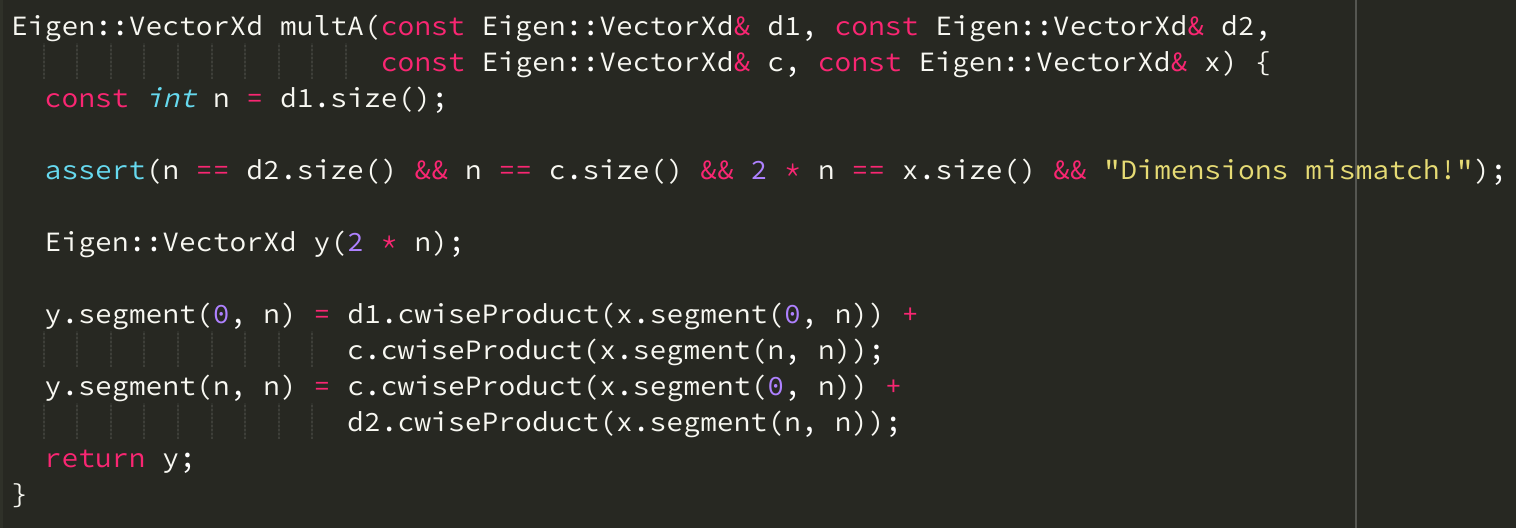
\includegraphics[width=1.0\linewidth]{2-2.b.png}
\end{figure}

\noindent Here \verb|segment(startIndex, length)| takes a segment starting at the index specified by the first argument and has length specified by the second argument and it can be used on \verb|Eigen::VectorXd|.

\subsection*{2-2.c}
We are tasked with computing the LU-factors of $\mathbf{A}$, where we may assume that they exist. We here remember (can also be taken from the hint) the block LU-factorization given by
\begin{equation*}
    \begin{bmatrix}
        \mathbf{A}_{11} & \mathbf{A}_{12} \\
        \mathbf{A}_{21} & 
        \mathbf{A}_{22}
    \end{bmatrix}
    = \begin{bmatrix}
        \mathbf{I} & \mathbf{O} \\
        \mathbf{A}_{21}\mathbf{A}_{11}^{-1} & \mathbf{I}
    \end{bmatrix}
    \begin{bmatrix}
        \mathbf{A}_{11} & \mathbf{A}_{12} \\
        \mathbf{O} & \mathbf{S}
    \end{bmatrix}
    \quad \text{with} \quad \underbrace{\mathbf{S} = \mathbf{A}_{22}-\mathbf{A}_{21}\mathbf{A}_{11}^{-1}\mathbf{A}_{12}}_{\text{Schur complement}}
\end{equation*}
this translates to 
\begin{equation*}
    \begin{bmatrix}
        \mathbf{D}_{1} & \mathbf{C} \\
        \mathbf{C} & 
        \mathbf{D}_{2}
    \end{bmatrix}
    = \underbrace{\begin{bmatrix}
        \mathbf{I} & \mathbf{O} \\
        \mathbf{C}\mathbf{D}_{1}^{-1} & \mathbf{I}
\end{bmatrix}}_{=\mathbf{L}}
    \underbrace{\begin{bmatrix}
        \mathbf{D}_{1} & \mathbf{C} \\
        \mathbf{O} & \mathbf{S}
    \end{bmatrix}}_{=\mathbf{U}}
    \quad \text{with} \quad \mathbf{S} = \mathbf{D}_{2}-\mathbf{C}\mathbf{D}_{1}^{-1}\mathbf{C}
\end{equation*}
Computing $\mathbf{D}^{-1}$ is simplified by the fact that $\mathbf{D}^{-1}$ is diagonal and we can thus for $\mathbf{D} = \text{diag}\left(d_{1}, \dots, d_{n}\right)$ compute $\mathbf{D}^{-1} = \text{diag}\left(\frac{1}{d_{1}}, \dots, \frac{1}{d_{n}}\right)$. We must now be careful when computing the matrix products as they would take $\mathcal{O}\left(n^{3}\right)$, but we can set up a zero matrix in $\mathcal{O}\left(n^{2}\right)$ and then compute the actual product in $\mathcal{O}\left(n\right)$, because we only have to compute it for the diagonal elements as all others will remain zero. Let us visualize this in a small example.

\begin{align*}
&\phantom{
    \begin{bmatrix}
        1 & 0 & 0 \\
        0 & 2 & 0 \\
        0 & 0 & 3
    \end{bmatrix}}\hspace{16px}
    \begin{bmatrix}
        \color{green}b_{1}\color{black} & 0 & 0 \\
        0 & \color{red}b_{2}\color{black} & 0 \\
        0 & 0 & \color{blue}b_{3}\color{black}
    \end{bmatrix} \\ 
    &\begin{bmatrix}
        \color{green}a_{1}\color{black} & 0 & 0 \\
        0 & \color{red}a_{2}\color{black} & 0 \\
        0 & 0 & \color{blue}a_{3}\color{black}
    \end{bmatrix}
    \begin{bmatrix}
        \color{green}c_{1}\color{black} & 0 & 0 \\
        0 & \color{red}c_{2}\color{black} & 0 \\
        0 & 0 & \color{blue}c_{3}\color{black}
    \end{bmatrix}
\end{align*}
the colours signify which entries in $\mathbf{A}$ and $\mathbf{B}$ contribute to entries in $\mathbf{C}$. We have
\begin{equation*}
    c_{1} = a_{1}b_{1} \quad c_{2} = a_{2}b_{2} \quad c_{3} = a_{3}b_{3}
\end{equation*}
hence only one multiplication per diagonal entry, we can do this operation in Eigen using \verb|cwiseProduct| for the diagonals of $\mathbf{A}$ and $\mathbf{B}$. This results in the following code.

\begin{figure}[!hbt]
    \centering
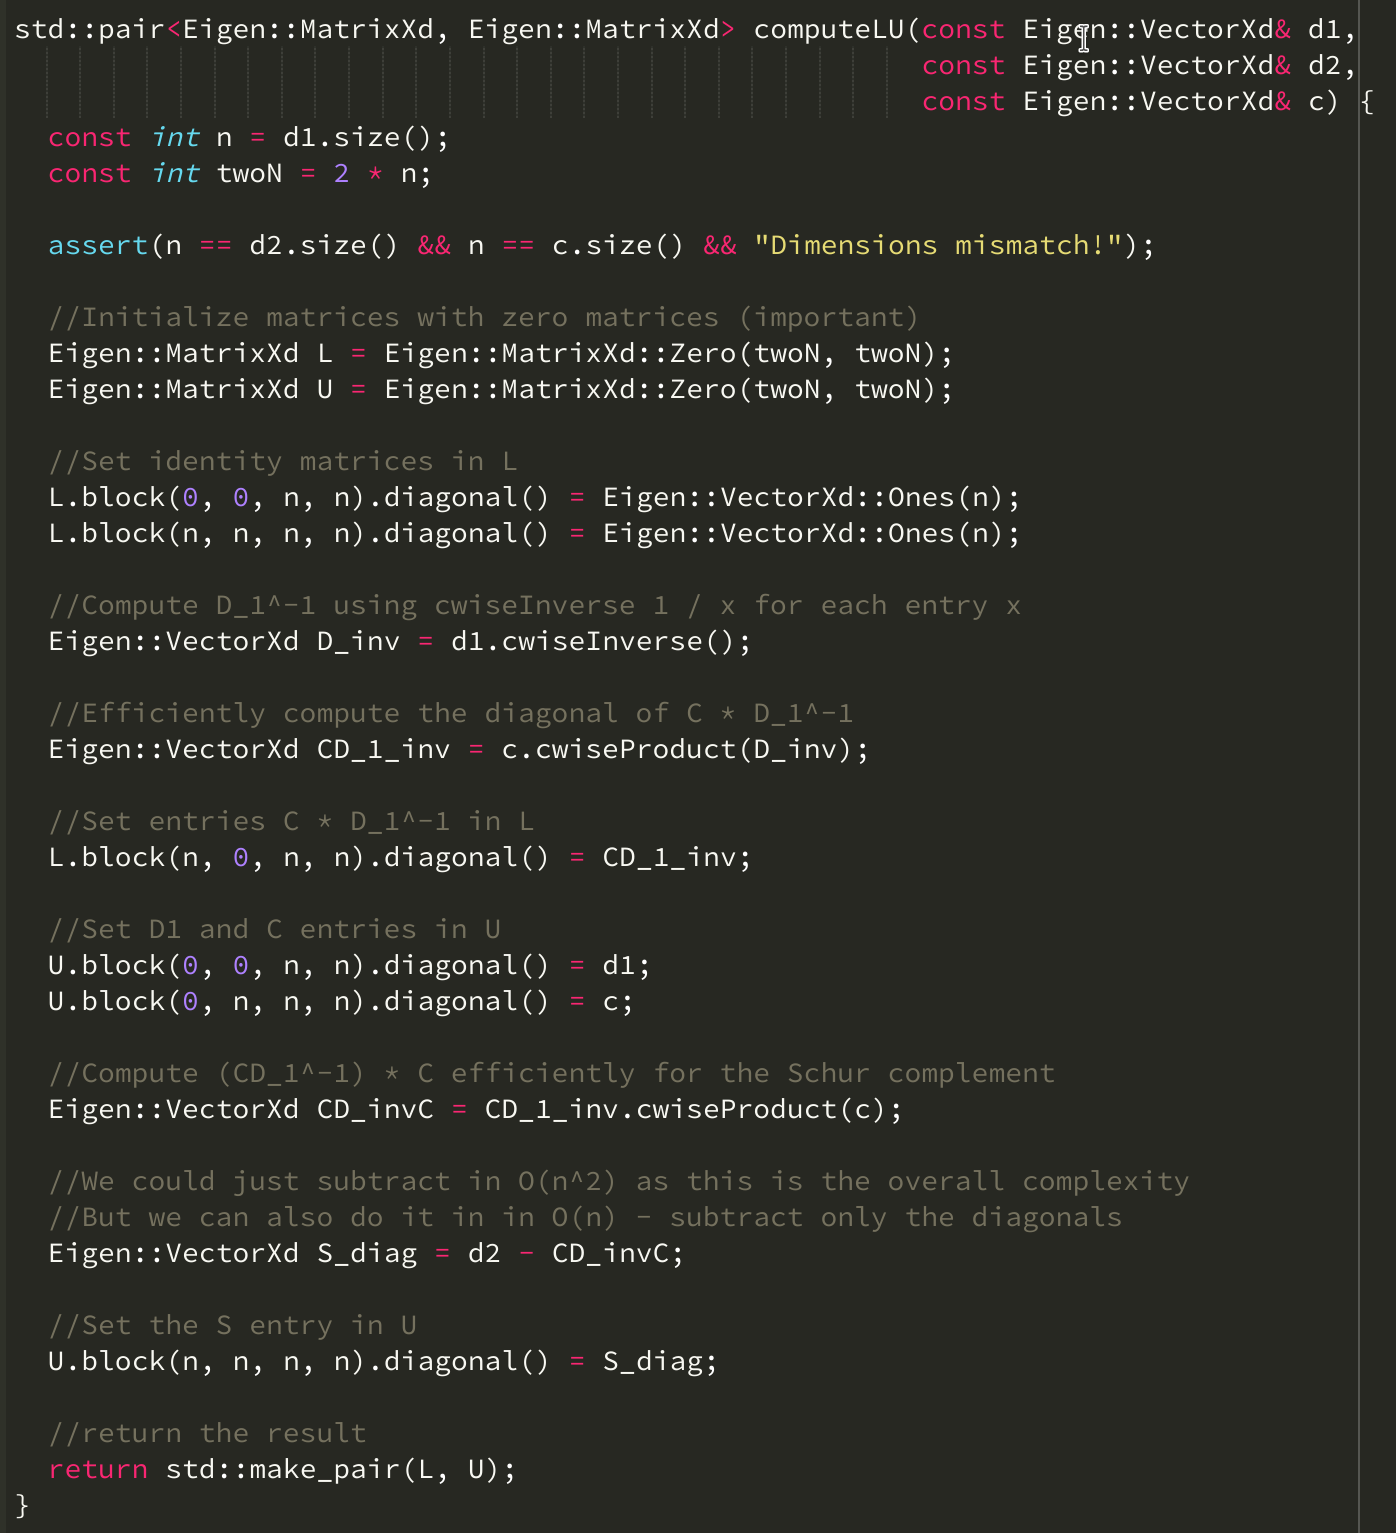
\includegraphics[width=0.7\linewidth]{2-2.c.png}
\end{figure}

\pagebreak

\noindent We could even make this better by storing the matrices $\mathbf{L}$ and $\mathbf{U}$ in one single matrix using the following format.

\begin{figure}[!hbt]
    \centering
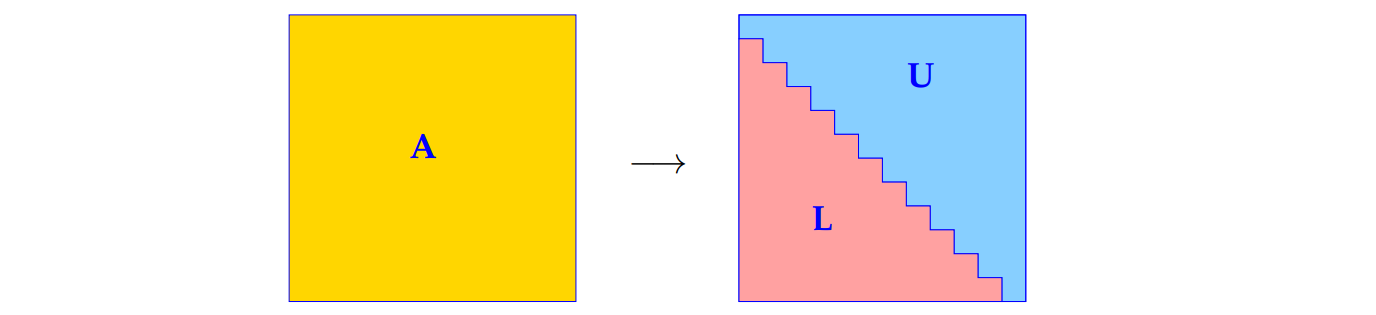
\includegraphics[width=1.0\linewidth]{LUStorage.png}
\end{figure}

\noindent where the $1$s one the diagonal of $\mathbf{L}$ are implied and are left out. We use for this purpose \verb|triangularView| in combination with the access modifiers \verb|Eigen::Upper| and \verb|Eigen::StrictlyLower| to access these matrices. This would then look like
\begin{figure}[!hbt]
    \centering
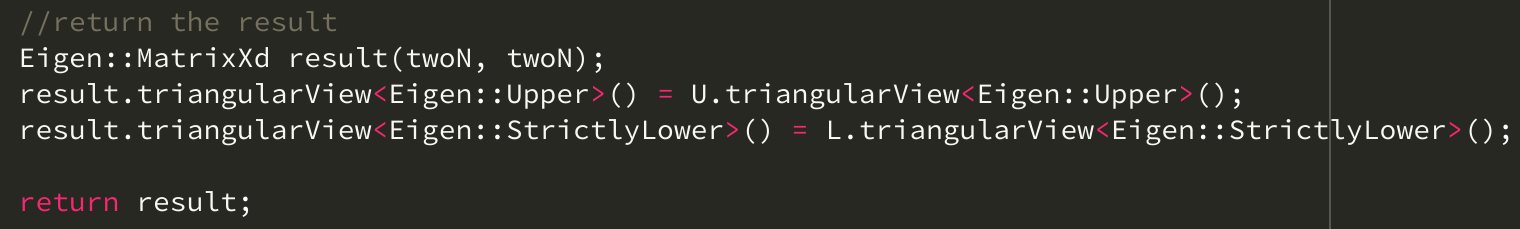
\includegraphics[width=1.0\linewidth]{StorageLU.png}
\end{figure}

\noindent and accessing the parts we could do via

\begin{figure}[!hbt]
    \centering
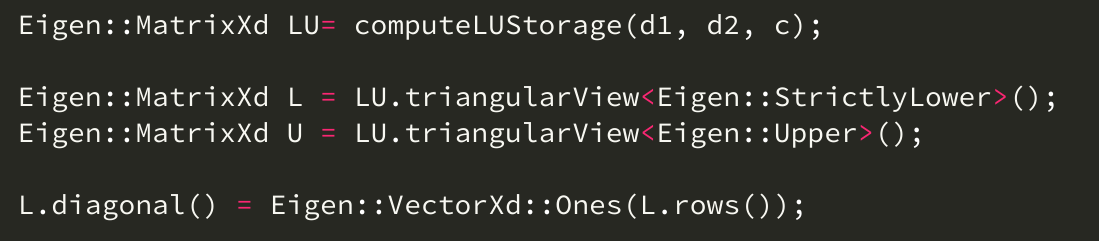
\includegraphics[width=0.8\linewidth]{AccessStorageLu.png}
\end{figure}

\subsection*{2-2.d}
We are now tasked with writing an efficient function \verb|solveA| that solves the system $\mathbf{A}\mathbf{x} = \mathbf{b}$. We have seen that we can decompose the coefficient matrix $\mathbf{A}$ into a modified tridiagonal matrix $\tilde{\mathbf{A}}$ that is composed of $2 \times 2$ blocks. We can solve these blocks separately and solve the entire system like that. The blocks where given by

\begin{equation*}
    \mathbf{B}_{i, \text{odd}} = \begin{bmatrix}
        d_{1, i} & c_{i} \\
        c_{i} & d_{2,i}
    \end{bmatrix} \quad
    \mathbf{B}_{i, \text{even}} = \begin{bmatrix}
        d_{2, i} & c_{i} \\
        c_{i} & d_{1,i}
    \end{bmatrix}
\end{equation*}
We must now must consider what happens to the system $\mathbf{A}\mathbf{x} = \mathbf{b}$ when we swap rows and columns of the coefficient matrix. If we switch rows, we must also switch the corresponding entries of $\mathbf{b}$ as we normally do in the Gaussian elimination. Switching columns on the other hand does not affect the right-hand side vector $\mathbf{b}$, it does however affect which column corresponds to which $x_{i}$ (entry of $\mathbf{x}$) and hence we must swap the corresponding entries in the vector $\mathbf{x}$.

\pagebreak

\noindent Let us observe this behaviour in a small example. 

\begin{equation*}
    \begin{bmatrix}
        d_{1,1}  & 0 & c_{1}  & 0 \\
        \mathbf{0} & \mathbf{d_{1,2}}  & \mathbf{0} & \mathbf{c_{2}}  \\
        \mathbf{c_{1}} & \mathbf{0} & \mathbf{d_{2,1}} & \mathbf{0} \\
        0 & c_{2}  & 0 & d_{2,2}  
    \end{bmatrix}\begin{bmatrix}
        x_{1} \\x_{2} \\x_{3} \\ x_{4}
    \end{bmatrix} =
    \begin{bmatrix}
        b_{1} \\ \mathbf{b_{2}} \\ \mathbf{b_{3}} \\ b_{4}
    \end{bmatrix} \longrightarrow \begin{bmatrix}
        d_{1,1}  & 0 & c_{1}  & 0 \\
        c_{1} & 0  & d_{2,1} & 0  \\
        0 & d_{1,2} & 0 & c_{2}\\
        0 & c_{2}  & 0 & d_{2,2}  
    \end{bmatrix}\begin{bmatrix}
        x_{1} \\x_{2} \\x_{3} \\ x_{4}
    \end{bmatrix} =
    \begin{bmatrix}
        b_{1} \\ b_{3} \\ b_{2} \\ b_{4}
    \end{bmatrix}
\end{equation*}

\begin{equation*}
    \begin{bmatrix}
        d_{1,1}  & \mathbf{0} & \mathbf{c_{1}}  & 0 \\
        c_{1} & \mathbf{0}  & \mathbf{d_{2,1}} & 0  \\
        0 & \mathbf{d_{1,2}} & \mathbf{0} & c_{2}\\
        0 & \mathbf{c_{2}}  & \mathbf{0} & d_{2,2}  
    \end{bmatrix}\begin{bmatrix}
        x_{1} \\ \mathbf{x_{2}} \\ \mathbf{x_{3}} \\ x_{4}
    \end{bmatrix} =
    \begin{bmatrix}
        b_{1} \\ b_{3} \\ b_{2} \\ b_{4}
    \end{bmatrix} \longrightarrow \begin{bmatrix}
        d_{1,1}  & c_{1} & 0  & 0 \\
        c_{1} & d_{2,1}  & 0 & 0  \\
        0 & 0 & d_{1,2} & c_{2}\\
        0 & 0  & c_{2} & d_{2,2}  
    \end{bmatrix}\begin{bmatrix}
        x_{1} \\ x_{3} \\ x_{2} \\ x_{4}
    \end{bmatrix} =
    \begin{bmatrix}
        b_{1} \\ b_{3} \\ b_{2} \\ b_{4}
    \end{bmatrix}
\end{equation*}

which then gives us the two linear systems we can solve seperately.
\begin{equation*}
    \begin{bmatrix}
        d_{1,1} & c_{1} \\
        c_{1} & d_{2,1}
    \end{bmatrix}
    \begin{bmatrix}
        x_{1} \\
        x_{3}
    \end{bmatrix} = 
    \begin{bmatrix}
        b_{1} \\
        b_{3}
    \end{bmatrix} \quad \begin{bmatrix}
        d_{1,2} & c_{2} \\
        c_{2} & d_{2,2}
    \end{bmatrix} \begin{bmatrix}
        x_{2} \\
        x_{4}
    \end{bmatrix} = 
    \begin{bmatrix}
        b_{2} \\
        b_{4}
    \end{bmatrix}
\end{equation*}
this does not allow us to predict the structure of a general system, let us hence look at the next bigger system.

\begin{align*}
    \begin{bmatrix}
        d_{1,1}  & \mathbf{0} & 0 & \mathbf{c_{1}}  & 0 & 0 \\
        0 & \mathbf{d_{1,2}} & 0  & \mathbf{0} & c_{2}  & 0 \\
        0 & \mathbf{0} & d_{1,3} & \mathbf{0} & 0 & c_{3} \\
        c_{1} & \mathbf{0} & 0& \mathbf{d_{2,1}} & 0 & 0 \\
        0 & \mathbf{c_{2}}  & 0 & \mathbf{0} & d_{2,2}  & 0 \\
        0 & \mathbf{0} & c_{3} & \mathbf{0} & 0 & d_{2,3}
    \end{bmatrix} \begin{bmatrix}
        x_{1} \\ \mathbf{x_{2}} \\ x_{3} \\ \mathbf{x_{4}} \\ x_{5} \\ x_{6}
    \end{bmatrix} = \begin{bmatrix}
        b_{1} \\ b_{2}\\ b_{3} \\ b_{4}\\ b_{5} \\ b_{6}
    \end{bmatrix} \\
    \longrightarrow\begin{bmatrix}
        d_{1,1}  & c_{1} & \mathbf{0} & 0 & \mathbf{0} & 0 \\
        0 & 0  & \mathbf{0} & d_{1,2} & \mathbf{c_{2}}  & 0 \\
        0 & 0 & \mathbf{d_{1,3}}& 0 & \mathbf{0} & c_{3} \\
        c_{1} & d_{2,1} & \mathbf{0}& 0 & \mathbf{0} & 0 \\
        0 & 0 & \mathbf{0} & c_{2} & \mathbf{d_{2,2}}  & 0 \\
        0 & 0 & \mathbf{c_{3}} & 0 & \mathbf{0} & d_{2,3}
    \end{bmatrix} \begin{bmatrix}
        x_{1} \\ x_{4} \\ \mathbf{x_{3}} \\ x_{2} \\ \mathbf{x_{5}} \\ x_{6}
    \end{bmatrix} = \begin{bmatrix}
        b_{1} \\ b_{2} \\ b_{3} \\ b_{4}\\ b_{5} \\ b_{6}
    \end{bmatrix} \\
    \longrightarrow \begin{bmatrix}
        d_{1,1}  & c_{1} & 0 & 0 & 0 & 0 \\
        \mathbf{0} & \mathbf{0}  & \mathbf{c_{2}} & \mathbf{d_{1,2}} & \mathbf{0}  & \mathbf{0} \\
        0 & 0 & 0& 0 & d_{1,3} & c_{3} \\
        \mathbf{c_{1}} & \mathbf{d_{2,1}} & \mathbf{0}& \mathbf{0} & \mathbf{0} & \mathbf{0} \\
        0 & 0 & d_{2,2} & c_{2} & 0  & 0 \\
        0 & 0 &0 & 0 & c_{3} & d_{2,3}
    \end{bmatrix}\begin{bmatrix}
        x_{1} \\ x_{4} \\ x_{5} \\ x_{2} \\ x_{3}\\ x_{6}
    \end{bmatrix} = \begin{bmatrix}
        b_{1} \\ \mathbf{b_{2}} \\ b_{3} \\ \mathbf{b_{4}}\\ b_{5} \\ b_{6}
    \end{bmatrix} \\
    \longrightarrow \begin{bmatrix}
        d_{1,1}  & c_{1} & 0 & 0 & 0 & 0 \\
        c_{1} & d_{2,1} & 0 & 0 & 0  & 0 \\
        0 & 0 & 0& 0 & d_{1,3} & c_{3} \\
        0 &0 & c_{2}& d_{1,2} & 0 & 0 \\
        0 & 0 & d_{2,2} & c_{2} & 0  & 0 \\
        0 & 0 &0 & 0 & c_{3} & d_{2,3}
    \end{bmatrix}\begin{bmatrix}
        x_{1} \\ x_{4} \\ x_{5} \\ x_{2} \\ x_{3}\\ x_{6}
    \end{bmatrix} = \begin{bmatrix}
        b_{1} \\ b_{4} \\ b_{3} \\ b_{2}\\ b_{5} \\ b_{6}
    \end{bmatrix}
\end{align*}

\pagebreak

\noindent We continue with the system from above

\begin{align*}
    \begin{bmatrix}
        d_{1,1}  & c_{1} & 0 & 0 & 0 & 0 \\
        c_{1} & d_{2,1} & 0 & 0 & 0  & 0 \\
        \mathbf{0} & \mathbf{0} & \mathbf{0}& \mathbf{0} & \mathbf{d_{1,3}} & \mathbf{c_{3}} \\
        0 &0 & c_{2}& d_{1,2} & 0 & 0 \\
        \mathbf{0} & \mathbf{0} & \mathbf{d_{2,2}} & \mathbf{c_{2}} & \mathbf{0}  & \mathbf{0} \\
        0& 0 &0 & 0 & c_{3} & d_{2,3}
    \end{bmatrix}\begin{bmatrix}
        x_{1} \\ x_{4} \\ x_{5} \\ x_{2} \\ x_{3}\\ x_{6}
    \end{bmatrix} = \begin{bmatrix}
        b_{1} \\ b_{4} \\ \mathbf{b_{3}} \\ b_{2}\\ \mathbf{b_{5}} \\ b_{6}
    \end{bmatrix} \\
    \longrightarrow 
    \begin{bmatrix}
        d_{1,1}  & c_{1} & 0 & 0 & 0 & 0 \\
        c_{1} & d_{2,1} & 0 & 0 & 0  & 0 \\
        0 & 0 & d_{2,2}& c_{2} & 0& 0 \\
        0 &0 & c_{2}& d_{1,2} & 0 & 0 \\
        0 & 0& 0 & 0 & d_{1,3}  & c_{3} \\
        0& 0 &0 & 0 & c_{3} & d_{2,3}
    \end{bmatrix}\begin{bmatrix}
        x_{1} \\ x_{4} \\ x_{5} \\ x_{2} \\ x_{3}\\ x_{6}
    \end{bmatrix} = \begin{bmatrix}
        b_{1} \\ b_{4} \\ b_{5} \\ b_{2}\\ b_{3} \\ b_{6}
    \end{bmatrix}
\end{align*}
This now gives us the following three $2 \times 2$ linear systems of equations.
\begin{equation*}
    \begin{bmatrix}
        d_{1,1} & c_{1} \\
        c_{1} & d_{2,1}
    \end{bmatrix} \begin{bmatrix}
        x_{1} \\ x_{4}
    \end{bmatrix} = \begin{bmatrix}
        b_{1} \\ b_{4}
    \end{bmatrix} \quad \begin{bmatrix}
        d_{2,2} & c_{2} \\
        c_{2} & d_{1,2}
    \end{bmatrix}\begin{bmatrix}
        x_{5} \\ x_{2}
    \end{bmatrix} = \begin{bmatrix}
        b_{5} \\ b_{2}
    \end{bmatrix} \quad \begin{bmatrix}
        d_{1,3} & c_{3} \\
        c_{3} & d_{2,3}
    \end{bmatrix} \begin{bmatrix}
        x_{3} \\
        x_{6}
    \end{bmatrix} = \begin{bmatrix}
        b_{3} \\ b_{6}
    \end{bmatrix}
\end{equation*}
We can now see that we will swap row / column $2$ with row / column $4$ resulting in the unknown $\left[x_{1},x_{4}\right]^{\mathsf{T}}$ and right-hand side $\left[b_{1},b_{4}\right]^{\mathsf{T}}$. Same goes for row / column $3$ and $5$, hence resulting in the unknown $\left[x_{3},x_{6}\right]^{\mathsf{T}}$ and right-hand side $\left[b_{3},b_{6}\right]^{\mathsf{T}}$. We will then get for the next unknown and right hand-side from the top
\begin{equation*}
    \begin{bmatrix}
        x_{i} \\ x_{2}
    \end{bmatrix} \quad \text{and} \quad \begin{bmatrix}
        b_{i} \\ b_{2}
    \end{bmatrix}
\end{equation*}
$i$ is determined by what the row / column $3$ was swapped with. We always swap the $j$-th row / column with the $j + 2$th row / column, hence this must mean that $i = 3 + 2$ and thus (in this case)
\begin{equation*}
    \begin{bmatrix}
        x_{5} \\ x_{2}
    \end{bmatrix} \quad \text{and} \quad \begin{bmatrix}
        b_{5} \\ b_{2}
    \end{bmatrix}
\end{equation*}
The goal is now to find the general structure of the $2$-vectors containing the $x_{i}$ and $b_{i}$. We will do this by building the $2 \times 2$ blocks we have seen before given by

\begin{equation*}
    \mathbf{B}_{i, \text{odd}} = \begin{bmatrix}
        d_{1, i} & c_{i} \\
        c_{i} & d_{2,i}
    \end{bmatrix} \quad
    \mathbf{B}_{i, \text{even}} = \begin{bmatrix}
        d_{2, i} & c_{i} \\
        c_{i} & d_{1,i}
    \end{bmatrix}
\end{equation*}

\pagebreak

We will denote in red colouring the element we would bring to the position marked in bold face. 

\begin{align*}
\begin{bmatrix}
        d_{1,1} & 0 & 0 & 0 & c_{1} & 0 & 0 & 0 \\
        0 & \mathbf{d_{1,2}} & 0 & 0 & 0 & c_{2} & 0 & 0 \\
         0 & 0& d_{1,3} & 0 & 0 &0 & c_{3} & 0\\
        0 & 0& 0 & d_{1,4} & 0 & 0 & 0 & c_{4} \\
        c_{1} & 0& 0 &0& \color{red}d_{2,1}\color{black}&0 & 0 & 0 \\
        0 & c_{2} & 0 & 0& 0 & d_{2,2} & 0 & 0 \\
        0 & 0& c_{3} & 0 & 0 & 0 & d_{2,3} & 0 \\
        0 & 0 & 0 &c_{4} & 0 & 0 & 0 & d_{2,4}
    \end{bmatrix}\begin{bmatrix}
        x_{1} \\ x_{2} \\ x_{3} \\ x_{4} \\ x_{5} \\ x_{6} \\ x_{7} \\ x_{8}
    \end{bmatrix} = \begin{bmatrix}
        b_{1} \\ b_{2} \\ b_{3} \\ b_{4} \\ b_{5} \\ b_{6} \\ b_{7} \\ b_{8}
    \end{bmatrix} \quad \substack{\text{swap column $2$ with column $5$} \\
                                  \text{swap row $2$ with row $5$}} \\
    \begin{bmatrix}
        \color{blue}d_{1,1}\color{black} & \color{blue}c_{1}\color{black} & 0 & 0 & 0 & 0 & 0 & 0 \\
        \color{blue}c_{1}\color{black} & \color{blue}d_{2,1}\color{black}& 0 &0& 0&0 & 0 & 0 \\
         0 & 0& d_{1,3} & 0 & 0 &0 & c_{3} & 0\\
        0 & 0& 0 & d_{1,4} & 0 & 0 & 0 & c_{4} \\
         0 & 0 & 0 & 0 & d_{1,2} & c_{2} & 0 & 0 \\
        0 & 0 & 0 & 0& c_{2} & d_{2,2} & 0 & 0 \\
        0 & 0& c_{3} & 0 & 0 & 0 & d_{2,3} & 0 \\
        0 & 0 & 0 &c_{4} & 0 & 0 & 0 & d_{2,4}
    \end{bmatrix}\begin{bmatrix}
        \color{blue}x_{1}\color{black} \\ \color{blue}x_{5}\color{black} \\ x_{3} \\ x_{4} \\ x_{2} \\ x_{6} \\ x_{7} \\ x_{8}
    \end{bmatrix} = \begin{bmatrix}
        \color{blue}b_{1}\color{black} \\ \color{blue}b_{5}\color{black} \\ b_{3} \\ b_{4} \\ b_{2} \\ b_{6} \\ b_{7} \\ b_{8}
    \end{bmatrix} \quad \phantom{\substack{\text{swap column $2$ with column $5$} \\
                                  \text{swap row $2$ with row $5$}}}                        
\end{align*}
This already gives us the first $2 \times 2$ linear system of equations (marked in bluw), we can hence ignore the top two rows and only look at the remaining rows. We proceed as before. In the following system we want to extract the block $\mathbf{B_{2}}$ and hence we could just implicitly do the swaps as the block is already given, we will do this properly though.
\begin{align*}
    \begin{bmatrix}
         d_{1,3} & 0 & 0 &0 & c_{3} & 0\\
        0 & d_{1,4} & 0 & 0 & 0 & c_{4} \\
          0 & 0 & \mathbf{d_{1,2}} & c_{2} & 0 & 0 \\
        0 & 0& c_{2} & \color{red}d_{2,2}\color{black} & 0 & 0 \\
        c_{3} & 0 & 0 & 0 & d_{2,3} & 0 \\
        0 &c_{4} & 0 & 0 & 0 & d_{2,4}
    \end{bmatrix}\begin{bmatrix}
         x_{3} \\ x_{4} \\ x_{2} \\ x_{6} \\ x_{7} \\ x_{8}
    \end{bmatrix} = \begin{bmatrix}
        b_{3} \\ b_{4} \\ b_{2} \\ b_{6} \\ b_{7} \\ b_{8}
    \end{bmatrix} \quad \substack{\text{swap column $3$ with column $4$} \\
                                  \text{swap row $3$ with row $4$}} \\
    \begin{bmatrix}
         d_{1,3} & 0 & 0 &0 & c_{3} & 0\\
        0 & d_{1,4} & 0 & 0 & 0 & c_{4} \\
        0 & 0& \color{blue}d_{2,2}\color{black} & \color{blue}c_{2}\color{black}& 0 & 0 \\
        0 & 0 & \color{blue}c_{2}\color{black}& \color{blue}d_{1,2}\color{black} & 0 & 0 \\
        c_{3} & 0 & 0 & 0 & d_{2,3} & 0 \\
        0 &c_{4} & 0 & 0 & 0 & d_{2,4}
    \end{bmatrix}\begin{bmatrix}
         x_{3} \\ x_{4} \\ \color{blue}x_{6}\color{black} \\ \color{blue}x_{2}\color{black} \\ x_{7} \\ x_{8}
    \end{bmatrix} = \begin{bmatrix}
        b_{3} \\ b_{4} \\ \color{blue}b_{6}\color{black} \\ \color{blue}b_{2}\color{black} \\ b_{7} \\ b_{8}
    \end{bmatrix} \quad \phantom{\substack{\text{swap column $3$ with column $4$} \\
                                  \text{swap row $3$ with row $4$}}}
\end{align*}
Extracting the $2 \times 2$ linear system of equations yields
\begin{align*}
     \begin{bmatrix}
         d_{1,3} & 0  & c_{3} & 0\\
        0 & d_{1,4} & 0 & c_{4} \\
        c_{3} & 0 & d_{2,3} & 0 \\
        0 &c_{4} &  0 & d_{2,4}
    \end{bmatrix}\begin{bmatrix}
         x_{3} \\ x_{4} \\ x_{7} \\ x_{8}
    \end{bmatrix} = \begin{bmatrix}
        b_{3} \\ b_{4}  \\ b_{7} \\ b_{8}
    \end{bmatrix}
\end{align*}

\pagebreak

\noindent We will now extract the last two $2 \times 2$ linear system of equations.

\begin{align*}
     \begin{bmatrix}
         d_{1,3} & 0  & c_{3} & 0\\
        0 & \mathbf{d_{1,4}} & 0 & c_{4} \\
        c_{3} & 0 & \color{red}d_{2,3}\color{black} & 0 \\
        0 &c_{4} &  0 & d_{2,4}
    \end{bmatrix}\begin{bmatrix}
         x_{3} \\ x_{4} \\ x_{7} \\ x_{8}
    \end{bmatrix} = \begin{bmatrix}
        b_{3} \\ b_{4}  \\ b_{7} \\ b_{8}
    \end{bmatrix}  \quad \substack{\text{swap column $2$ with column $3$} \\
                                  \text{swap row $2$ with row $3$}} \\
                                  \begin{bmatrix}
         \color{blue}d_{1,3}\color{black} & \color{blue}c_{3}\color{black}  & 0 & 0\\
         \color{blue}c_{3}\color{black} & \color{blue}d_{2,3}\color{black} & 0 & 0 \\
        0 & 0 & \color{orange}d_{1,4}\color{black} & \color{orange}c_{4}\color{black} \\
        0 &0&  \color{orange}c_{4}\color{black} & \color{orange}d_{2,4}\color{black}
    \end{bmatrix}\begin{bmatrix}
         \color{blue}x_{3}\color{black} \\ \color{blue}x_{7}\color{black} \\ \color{orange}x_{4}\color{black} \\ \color{orange}x_{8}\color{black}
    \end{bmatrix} = \begin{bmatrix}
        \color{blue}b_{3}\color{black} \\ \color{blue}b_{7}\color{black}  \\ \color{orange}b_{4}\color{black} \\ \color{orange}b_{8}\color{black}
    \end{bmatrix}  \quad \phantom{\substack{\text{swap column $2$ with column $3$} \\
                                  \text{swap row $2$ with row $3$}}}
\end{align*}
This gives us the last systems (we only need to swap rows / columns in the one on the lower right corner). Let us consider these systems now.
\begin{align*}
    \begin{bmatrix}
        d_{1,1} & c_{1} \\
        c_{1} & d_{2,1}
    \end{bmatrix} \begin{bmatrix}
        x_{1} \\ x_{5}
    \end{bmatrix} = \begin{bmatrix}
        b_{1} \\ b_{5}
    \end{bmatrix}
    \qquad \begin{bmatrix}
        d_{2,2} & c_{2} \\
        c_{2} & d_{1,2}
    \end{bmatrix}\begin{bmatrix}
        x_{6} \\ x_{2}
    \end{bmatrix} = \begin{bmatrix}
        b_{6} \\ b_{2}
    \end{bmatrix} \\[2mm]
    \begin{bmatrix}
        d_{1,3} & c_{3} \\
        c_{3} & d_{2,3}
    \end{bmatrix}\begin{bmatrix}
        x_{3} \\ x_{7}
    \end{bmatrix} = \begin{bmatrix}
        b_{3} \\ b_{7}
    \end{bmatrix} \qquad \begin{bmatrix}
        d_{2,4} & c_{4} \\
        c_{4} & d_{1,4}
    \end{bmatrix}\begin{bmatrix}
        x_{8} \\ x_{4} 
    \end{bmatrix} = \begin{bmatrix}
        b_{8} \\ b_{4}
    \end{bmatrix}
\end{align*}

\noindent We can rewrite these systems to (makes it easier to read of the general structure)
\begin{align*}
    \begin{bmatrix}
        d_{1,1} & c_{1} \\
        c_{1} & d_{2,1}
    \end{bmatrix} \begin{bmatrix}
        x_{1} \\ x_{5}
    \end{bmatrix} = \begin{bmatrix}
        b_{1} \\ b_{5}
    \end{bmatrix}
    \qquad \begin{bmatrix}
        d_{1,2} & c_{2} \\
        c_{2} & d_{2,2}
    \end{bmatrix}\begin{bmatrix}
        x_{2} \\ x_{6}
    \end{bmatrix} = \begin{bmatrix}
        b_{2} \\ b_{6}
    \end{bmatrix} \\[2mm]
    \begin{bmatrix}
        d_{1,3} & c_{3} \\
        c_{3} & d_{2,3}
    \end{bmatrix}\begin{bmatrix}
        x_{3} \\ x_{7}
    \end{bmatrix} = \begin{bmatrix}
        b_{3} \\ b_{7}
    \end{bmatrix} \qquad \begin{bmatrix}
        d_{1,4} & c_{4} \\
        c_{4} & d_{2,4}
    \end{bmatrix}\begin{bmatrix}
        x_{4} \\ x_{8} 
    \end{bmatrix} = \begin{bmatrix}
        b_{4} \\ b_{8}
    \end{bmatrix}
\end{align*}
\noindent We get the general structure for block size of $n$ (length of the vectors $c$, $d_{1}$ and $d_{2}$) using that for $n$ we get $n$ such systems and we must thus have an offset of $n$ between the $x_{i}$ and $b_{i}$ in the $2 \times 2$ systems to cover all elements.
\begin{equation*}
    \begin{bmatrix}
        d_{1,i} & c_{i} \\
        c_{i} & d_{2,i}
    \end{bmatrix}\begin{bmatrix}
        x_{i} \\ x_{i + n}
    \end{bmatrix} = \begin{bmatrix}
        b_{i} \\ b_{i + n}
    \end{bmatrix} \quad \text{for } 1 \leq i \leq n
\end{equation*}
the solution of these is then given by using the inverse of a $2 \times 2$ matrix being (if it exists)
\begin{equation*}
    \mathbf{A} = \begin{bmatrix}
        a & b \\
        c & d
    \end{bmatrix} \implies \mathbf{A}^{-1} = \frac{1}{ad - bc} \begin{bmatrix}
        d & -b \\
        -c & a
    \end{bmatrix}
\end{equation*}
and thus
\begin{equation*}
    \begin{bmatrix}
        x_{i} \\
        x_{i + n}
    \end{bmatrix} = \frac{1}{d_{1,i}d_{2,i} - c_{i}^{2}}\begin{bmatrix}
        d_{2,i} & -c_{i} \\
        -c_{i} & d_{1,i}
    \end{bmatrix}\begin{bmatrix}
        b_{i} \\ b_{i + n}
    \end{bmatrix}
\end{equation*}
We can thus compute this for all $1 \leq i \leq n$ and will have our solution. We must check if 
\begin{equation*}
    d_{1,i}d_{2,i} - c_{i}^{2} \neq 0
\end{equation*}
as otherwise the system has not solution (besides the one in the least squares sense).

\pagebreak

\noindent We will not use block matrices in our code as this would be inefficient we instead compute the result of the matrix-vector product and set the entries directly.

\begin{equation*}
    \begin{bmatrix}
        d_{2,i} & -c_{i} \\
        -c_{i} & d_{1,i}
    \end{bmatrix}\begin{bmatrix}
        b_{i} \\ b_{i + n}
    \end{bmatrix} = \begin{bmatrix}
        d_{2,i}b_{i} - c_{i}b_{i+n} \\
        -c_{i}b_{i} + d_{1,i}b_{i+n}
    \end{bmatrix}
\end{equation*}

This produces the following code.
\begin{figure}[!hbt]
    \centering
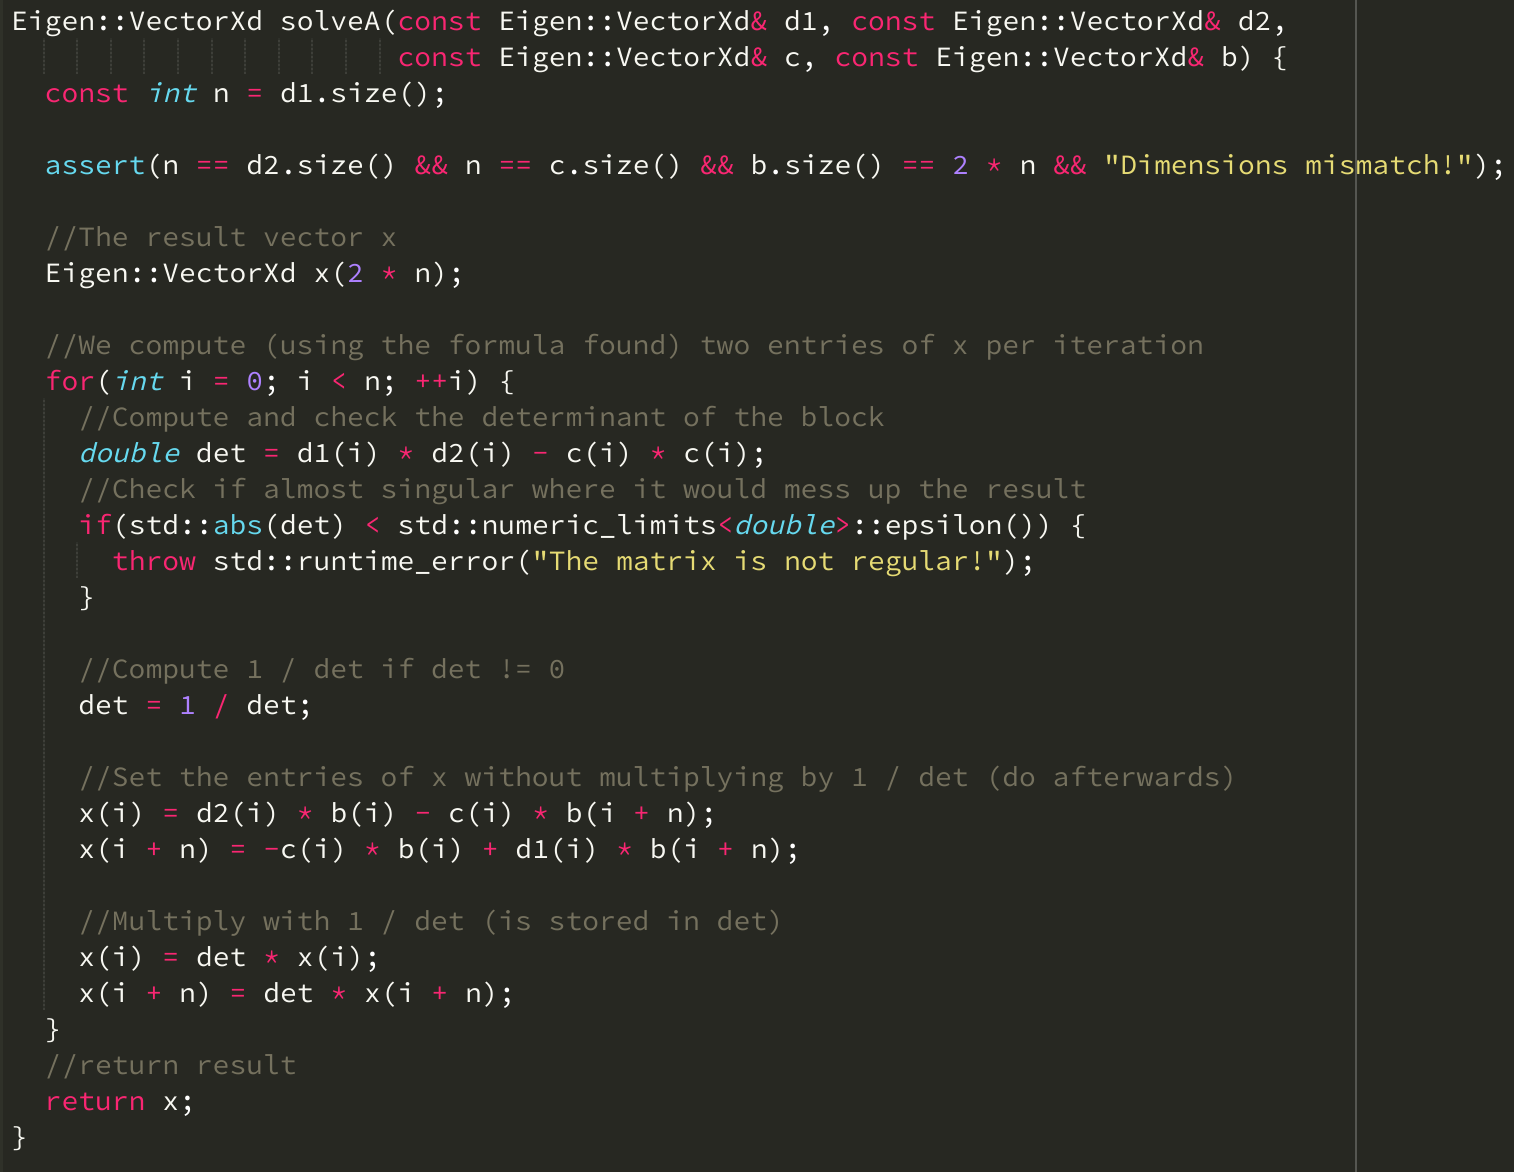
\includegraphics[width=1.0\linewidth]{2-2.e.png}
\end{figure}

\subsection*{2-2.e}
We are tasked with determining the asymptotic complexity of our code. Let us thus go through the code. We do $n$ iterations of the loop All the computations we do take $\mathcal{O}\left(1\right)$ time inside the loop. Hence overall we get a complexity of $\mathcal{O}\left(n\right)$.

\subsection*{2-2.f}
The timer utility in \verb|C++| uses and object of type \verb|Timer| and the methods \verb|start()| and \verb|stop()| to start / stop said timer. We then use \verb|duration()| (for single runs) to get the desired results. The given solution goes into detail here, hence no additional solution will be added here.

\end{document}
